\section{Versuchsaufbau}
\begin{figure}
	\centering
	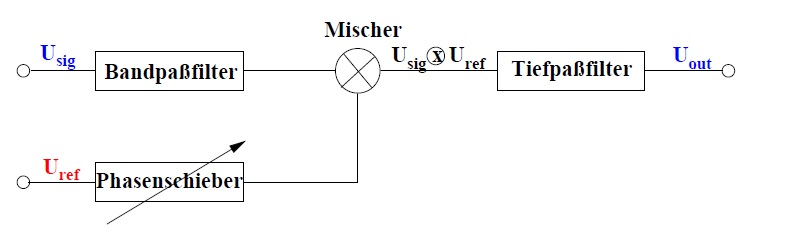
\includegraphics{../../Aufbau}
	\caption{Höppler Viskosimeter - Der Aufbau}
	\label{fig:aufbau}
\end{figure}
In der Abbildung \ref{fig:aufbau} ist der Aufbau nach Höppler-Viskosimeter zu sehen. Die Libelle dient zur Justifizierung des Viskosimeters, so dass das gerade stehen soll. Das Fallrohr hat mehrere Meßmarken und befindet sich in einem Wasserbad, wo das Wasser zuerst eine konstante Temperatur besitzt. In das Fallrohr kann die zu untersuchende Kugel eingegeben und Wasser gefüllt werden. Wenn die Kugel in das Fallrohr eingegeben wird, muss das Rohr durch eine Schraube verschlossen sein. Die Temperatur kann durch einen Thermostat erhitzt werden und mit Hilfe von einem Thermometer an dem Viskosimeter abgelesen werden.
\section{Durchführung}
\label{sec:Durchführung}
Als erstes wird jeweils fünf mal der Durchmesser für die kleine und große Kugel gemessen. Danach wird mit Hilfe der Libelle das Viskosimeter so justiert, dass das gerade stehen kann. Als nächstes wird das Rohr mit destilliertem Wasser gefüllt und die Luftblasen mit einem Holzstab herausgenommen. Der kleine Kugel wird zuerst in das Rohr vorsichtig eingeworfen, so dass es erneut keine Luftblasen entstehen können. Letztendlich wird das Rohr mit einer Schraube verschlossen. Das Viskosimeter wird um $\SI{180}{\degreeCelsius}$ gedreht und mit einem manuellen Stoppuhr die Zeit für 10 Messungen bestimmt. Vor dem Passieren der ersten Meßmarke stellt sich eine konstante Geschwindigkeit $v$ der Kugel. Es wird die Zeit gemessen, die die Kugel von der ersten Meßmarke bis zur letzten Meßmarke braucht. Während dieses Vorgangs besitzt die Kugel immer noch eine konstante Geschwindigkeit. Die kleine Kugel wird vorsichtig herausgenommen und neues distilliertes Wasser in das Rohr gefüllt. Dieser Vorgang wird auch mit der großen Kugel wiederholt. 
Für die nächste Durchführung wird die große Kugel nicht entfernt. Das Fallrohr befindet sich in einem Wasserbad, das mit Hilfe von einem Thermostaten bis zu $\SI{70}{\degreeCelsius}$ aufgeheizt werden kann und mit einem Thermometer die zugehörige Temperatur abgelesen werden kann. Für 10 verschiedene Temperaturen, wird die Fallzeit zwei Mal der großen Kugel gemessen also das Viskosimeter wird jeweils zwei Mal um $\SI{180}{\degreeCelsius}$ gedreht.
 